\documentclass{article}
\usepackage{amsmath, amsthm, amssymb, amsfonts, bm}
\usepackage{graphicx}
\usepackage[T1]{fontenc}
\usepackage[utf8]{inputenc}
\usepackage[a4paper]{geometry}
\usepackage{fancyhdr}
\usepackage[algo2e]{algorithm2e}
\fontfamily{cmr}

\title{DD2424 - Assignment 4}
\author{Oskar Stigland \\ stigland@kth.se}

\pagestyle{fancy}
\fancyhf{}
\rhead{stigland@kth.se}
\lhead{DD2424 - Deep Learning in Data Science}
\rfoot{Page \thepage}

\begin{document}
%\maketitle

	\begin{titlepage}
		\begin{center} 
			
			\rule{\linewidth}{0.5mm}\\[0.5 cm]
			{ \huge \bfseries DD2424 - Assignment 4}\\[0.3 cm] % Title of your document
			\rule{\linewidth}{0.5mm}\\[1 cm]
					
			\small\vfill
			\begin{center}
			\centering
			{\large \bfseries \textsc{Summary}}\\
			\vspace{1cm}
			\begin{minipage}{10cm}
				
				I have verified the analytical gradients for the $1$-layer RNN and they seem to be correct. I have then proceeded to train the network for some $100$ thousand steps, producing text sequences at every $10$ thousand steps and checking the evolution of the generated text sequences. Finally, a network is trained for a longer period, specifically $4$ epochs, and then a longer sequence is produced with the weights that achieved the lowest loss.\\\\
%
	The code for the assignment has been written in \texttt{python}. I have implemented the neural network as a class. For the hand-in, all of the code has been put toghether in a main file with all the functions and the class declared at the top. For the hand-in, I have also commented out the saving of generated figures and results in JSON files, as well as omitting some of the case-specific testing and gradient testing.
			\end{minipage}
			\end{center}
			\large\vfill
						

		\end{center}	
		
		\begin{minipage}{0.4\textwidth}
			\begin{flushleft} \large
				%\emph{Student:}\\
				Oskar \textsc{Stigland}\\
				DD2424\\
				Spring 2023
			\end{flushleft}
		\end{minipage}	

	\end{titlepage}

\newpage

\subsection*{Checking gradients}

	In order to validate the anaytic gradient computations, I compared the analytically computed gradients with numerically computed gradients on a large subset of the weights for a number of different sequential inputs, using $h = 10^{-5}$.  I got that
	$$\vert\vert \nabla_{\bm{w}} \bm{J}- \nabla_{\bm{w}} \bm{J}^{\text{numerical}} \vert\vert_{\infty} < 10^{-8}, \quad \forall\bm{w} \in \bm{W}, \bm{V}, \bm{U}, \bm{b} ,\bm{c}$$
	More specifically, I checked $50\times50$ weights for $\bm{W}, \bm{V}, \bm{U}$ and $50$ weights for $\bm{b} ,\bm{c}$. I ran the same test for a number of sequences and consistently achieved an error on the order of $10^{-8}$. I also attempted to train the network for a number of epochs in order to see the behavior of the loss function. I initially tried to train it on just a small subset of the data, using only a couple of thousand sequences and training for a shorter number of iterations. However, it was difficult to find a seemingly sensible combinations of subset size and number of iterations. Rather, I used the entire set of sequences and trained for some $30$ thousand iterations. I initiated the smooth loss with the loss computed with the untrained network on the first sequence. The results are plotted below. The network seems to converge fairly quickly to a pleateau. Hence, given the proximity of numerially and analytically computed gradients, I am confident that the gradients are indeed correctly specified.
	\begin{figure}[h!]
		\centering
		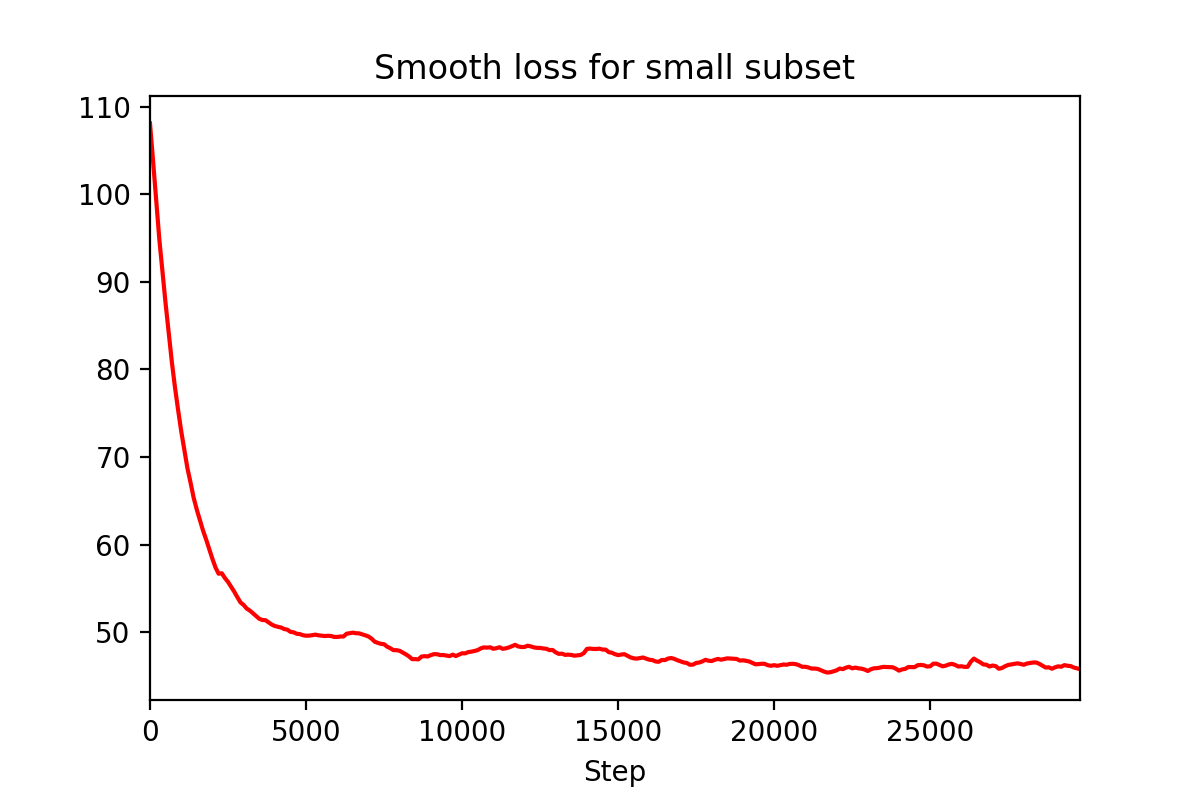
\includegraphics[width=12cm]{../plots/grad_test_rnn.png}
		\caption{Loss for $1$-layer recurrent neural network with $m=100$, trained for a shorter period and some $30$ thousand steps.}
 	\end{figure}

\newpage
\subsection*{Training the RNN}

\subsubsection*{Results for a long-ish training period}
	I trained the $1$-layer RNN for a longer training period with $\eta = 0.1$. I evaluated the smoothed loss at every step, which was initiated as the loss for the untrained network on the first training example in the set of sequences - and compared the loss to a "best" loss in order to find the best network. I then saved the smooth loss at every $10$ steps. The loss seems to converge fairly quickly to a plateau around $40-45$. The results are shown below for $4$ epochs of training:

	\begin{figure}[h!]
		\centering
		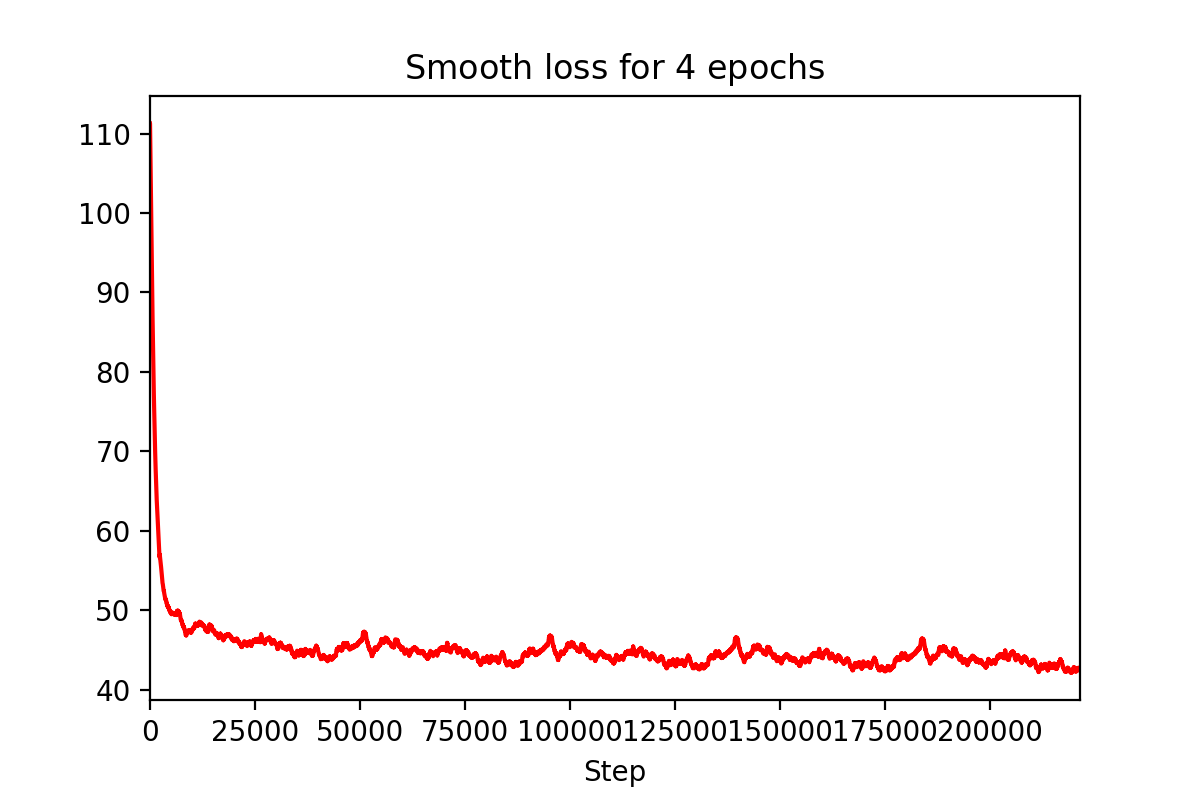
\includegraphics[width=12cm]{../plots/rnn_loss.png}
		\caption{Loss for $1$-layer recurrent neural network with $m=100$, trained for $4$ epochs.}
 	\end{figure}

\subsubsection*{Producing a longer sequence}
	After training the network for $4$ epochs, I generated a longer sequence of text using the network weights which achieved the lowest loss:
	\begin{quote}
		\smaller
		AKTHerdss to be eny\'s Mast heaving the Galled their it inde.  Ast, I laressed of hadremone of of Voldemort.\\
		"What yell, he at a mett liken, bremp as the atpertise, Hermione when comecter they halling a who did exer Dupped, as the Drastered," Foncum on the hawry to Fook, yeas, he said stive ioming see," Hermione of peel," heard.  The manicingorn, are would had told."\\
		"Harry, where.  So the Gat into meaved it.\\
		"And mo it been time was get a his looked a now who disted yavengeling.\\
		"Sight," the glasterly.\\
		"Their toly.  Harry on was in this, as the on I zarry\'s had maless to hears.  Harry, nowwask.\\
		"My the devernon to poinvenem?"\\
		"Oly prath Pruffne wied yourne worn frisicould, and Ead poldes wand follly of look, but but the the - Fudge lins.\\
		"Think do knowdly him munded as Krum pidned you light, thoughs agains ung well his when isle all Cedling.  He as them say.  They great it, as Gratch and so Dumanly, hil do I pably, and quils Toint inteld with I votiou in the first him cuttey was have at
	\end{quote}

\newpage
\subsection*{Generated sequences}

\subsubsection*{Steps: 0}
\begin{quote}
	\smaller
	AXO6"iH2jLL,T1;¢iDdz	6Kjâ(R2/lE:JkHI6oqgs2zbZuQI-t(\_)L9n\^cnEMEF/LziWjEhJJm\\3GKoLXZDiHj-y€sFXqbE;dpb!0kf€LvEpN6WNd\_k;p
	gZksib?kEL€z)Yo-¢Câ7/ GyI\^N\\(:jn"YJ(vL9Ãd¢HO6,VCrINfRE4kROb?.smLDZV7U7âtV/fVÃEX'?Vs3EUjKM6YJ\\YJ1Ol"tEWU),YEvb\^jEND)TXZE¢"k"4TUl?pEcZ4\_Sl
\end{quote}

\subsubsection*{Steps: 10000}
\begin{quote} 
	\smaller
	C Werealilnmarry druthawadd cnukearding haddsann thick."\\
	"vented they- th. Durry a Kanmy ballaa hin pre asly. .Hoon hurry be to tore Hare theme terchre kam Das - ."\\
	Sure theme rack was the mard alt surring baid al hin was on'rmittnave glane to R't ksm
\end{quote}

\subsubsection*{Steps: 20000}
\begin{quote} 
	\smaller
	re as a ding bres his they'g madeytle whicking?" ser stanx the coulln't anby was of his boy's the shay.. Goleens.  "Hor and S ickert the in . .  We leool, ado't meriest of Hagior - was - feving from in and and wappsbroy riching he wark have foleatess
\end{quote}

\subsubsection*{Steps: 30000}
\begin{quote} 
	\smaller
	lough hindy and "llongherster lyed hack cowd the ando ever s into his grome the forethly, of mrgpobe priglly deros lit.  Theballw to his ferter the siphed getur. They treat.
	Harrshe's even fir.\\\\
	%
	Harry slout ont - yoh fereg to herng, was ntercenoring t
\end{quote}

\subsubsection*{Steps: 40000}
\begin{quote}
	\smaller
	nod - into .  Ho armund not twand wavered; store, and stenys in, he waster told as wack right girent. . . ..this fanterny!  Veble summed, looked  fend Visting frase creagraky, 		betthing rooped and wase, to net the cates casts in the stase corn's waid t
\end{quote}

\subsubsection*{Steps: 50000}
\begin{quote}
	\smaller
	to that the MaveNzincen to down polkss said, Magieey I then g. RThem, comble wanding the Ozu-drofuladst thing dide fanted moads and beans wanly.
	"Fou dantebn us all a nothing rears thentwny chy, reem all reang sald shand.  I very gilistarts shise...
\end{quote}

\subsubsection*{Steps: 60000}
\begin{quote}
	\smaller
	ong was sarstuing as had stray-Knofage of Most yous it you," said Ron, fapsing all yived awry hall tretsen terturenther, tho tS nught his fidn't lot's. "Pargs has whestseary at tsey yeag, I mowt herrangers.\\
	"Harry. "The rilion, "Hagiin. "You her skire
\end{quote}

\subsubsection*{Steps: 70000}
\begin{quote}
	\smaller
	e chear outd, gut shoeddan into, we cake thimblecopenyouldered his's..  Prry do the warkey, cemaling that?" Nadn very chome seenous and in thes, you next but Toners-lecoman cank I conking thought lehel shink aloning quids Son," he owf doned her coning
\end{quote}

\subsubsection*{Steps: 80000}
\begin{quote}
	\smaller
	n lye, torf aboo Moode.  ". Wutt Ron, inde in timindol again Mr. WHoparn.  YGard that. He were loom.  I bach on aboom.
	"The migatay now in mut hearing as madmasced it dedread he wasted.  "Yemen hingwly was that Ron. Lointwaingarad back he - we was to
\end{quote}

\subsubsection*{Steps: 90000}
\begin{quote}
	\smaller
	le, it, now; all finly, wisn't word, and had did, at - exontped voite ton, whins, and and segfed fores a serting head had theo his for Ardor horres in Magou hollist iodn't befueply's frond be snide's it, Lord-rhatted wizard clawn for stiple hap ochean
\end{quote}

\subsubsection*{Steps: 100000}
\begin{quote}
	\smaller
	t with peated alod Dumbledored of his chill beoney trincy be ongry co that uf they Aee eeteh the eiving to befad," said Hermione sow stront dove wop off toldy fellowcly, anding cinky the rose to the ol.\\
	hiss you." Ehe, Dumbleded of mory?"  them!"\\
	"Th
\end{quote}
\end{document}